\documentclass[12pt]{article}
\usepackage{wkrpt}
\begin{document}


\title{Analysis of Web Application Functional Testing Options}
{
	Telus Health Inc.\\
	Mississauga, ON L4W 4T9
}
{
	\textbf{Prepared by}\\[2ex]
	
	Daiwei Fan\\
	Student ID: 20458752\\
	User ID: d3fan\\
	2A Software Engineering\\
	April 11, 2014
}


\letter{Analysis of Web Application Functional Testing Options}{first}{2A}{Telus Health Inc.}
{
	\noindent
	Daiwei Fan\\
	\#48, 461 Beechwood Place\\
	Waterloo, ON\\
	N2T 2N8
}
{
	Telus Health provides health and related transaction record for clients of medical insurance companies. I was situated in the new VIP room team, which is responsible for rebuilding a web service for clients to look up their drug claim transaction history. During my time in Telus, I was assigned to study the pre-existing interface and to extract data from existing log files.
}
{
	The following report performs an analysis on the different techniques for testing features implemented in VIP room. This problem is one that I encountered during my work term. My team had to decide which method was best suited to the task given all the requirements and our abilities.
}
{
	I would like to thank my manager Kevin Ho and Quality Analyst Anshuman Ghandi, both of whom gave inputs on how functionality testing is done in other projects produced by Telus Health.
}
{
	Daiwei Fan\\
	Student ID: 20458752\\[2ex]
	Encl.
}


\tocsection{Executive Summary}
EXECUTIVE SUMMARY



\newpage

\toc
% \lof
% \lot


\pagenumbering{arabic}
\section{Introduction}

Telus Health is a “TELUS Health is a leader in telehomecare, electronic medical and health records, consumer health, benefits management and pharmacy management.”\cite{telusComp}. With the recent acquisition of Med Access Inc., Telus is “confirmed as the largest EMR (Electronic Medical Record) provider in Canada”\cite{telusComp}. This title has encouraged Telus to provide service with higher quality. In January 2014, I was assigned to the VIP room to implement a web service that mainly contains a drug claim searching and benefit management feature. This particular feature allows different levels of users such as patient, insurer and pharmacist to access the patient's record of drug claims and payments. After a certain amount of designing and coding, it came to the point where some basic testing for the code was necessary. I believe that even elementary testings should be carefully designed for future documentation and reproduction. \\

Functionality testing has always been one of the most important tasks in the quality assurance (abbreviated as QA) process. All companies are working to discover a testing method which is able to cover all sources of error, requires minimal human effort and consumes least amount of time. It is especially important for Telus Health, a company which has adapted the Agile software development system, to have a highly efficient QA process in order to accommodate the fast pace of the system. At Telus, agile development is structured as series of “sprint cycles.” Every aspect of the development process, including technical requirements, design etc., are continually revisited throughout the lifecycle of the project. As a consequence, a series of developing and testing will take place. As illustrated in Figure 1, the testing phase appears on a intense frequency, which results in many high demands on the tests' quality, efficiency etc. These demands will be considered as criteria to evaluate a testing approach later on in the report.\\

\begin{figure}[ht!]
\centering
\includegraphics[width=12.5cm,height=12.5cm,keepaspectratio]{img/agile.png}
\caption{Agile development workflow}
\label{overflow}
\end{figure}

This report provides an evaluation of three functionality testing methods, assessing their 
suitability to the VIP room web service. You will first be introduced to the VIP room work flow. Then, the three approaches for testing will be explained and compared in detail. Comparisons will be made among various criteria and will be finalized using the Decision Matrix Analysis. Finally, the report summarizes the results of the analysis, draws 
conclusions, and makes a recommendation. The reader is expected to have reasonable background in web service development. Basic knowledge in the Extensible Markup Language (XML)would also help the reader quickly understand one of the approaches. Other technology and terminologies used in this report will be explained on their first appearance.\\



\newpage

\section{Problem Specification}
\subsection{Background}
The VIP room web service utilizes the traditional three-tier architecture. Figure 2 depicts the sequence diagram of a three-tier web service workflow:

\begin{figure}[ht!]
\centering
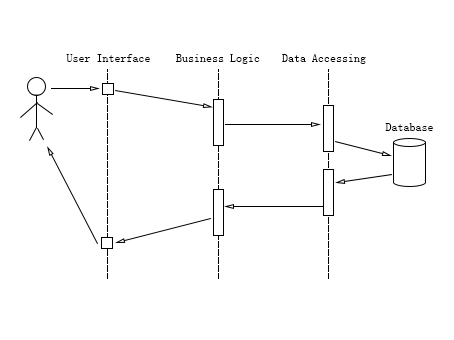
\includegraphics[width=12cm,height=12cm,keepaspectratio]{img/three_tier.jpg}
\caption{three-tier web service sequence diagram}
\label{overflow}
\end{figure}

\subsection{Options}
The three testing approaches sends data to different part of the flow.\\
\subsubsection{Manual testing from User Interface}
The most naive method is to manually enter input data on the User Interface (UI) \\
		
\begin{figure}[ht!]
\centering
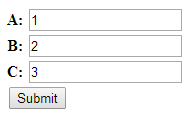
\includegraphics[width=7cm,height=7cm,keepaspectratio]{img/ui.jpg}
\caption{input from simple UI}
\label{overflow}
\end{figure}

\subsubsection{Simple Object Accessing Protocol (SOAP)}
	This method uses the Simple Object Accessing Protocol. "SOAP is a lightweight protocol for exchange of information in a decentralized, distributed environment."\cite{soap} It wraps the input data in an envelope and sends it as a request directly to the business layer. A soap request template is populated based on a file written in Web Services Description Language (WSDL). This file can be generated from a Java Class containing business logic. In most cases this Class is the controller or entrance to the business layer. The following is a screen shot of a SOAP client called “SoapUI”:
	
\begin{figure}[ht!]
\centering
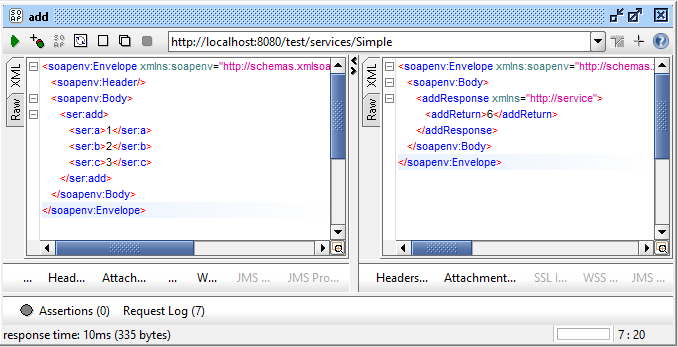
\includegraphics[width=15cm,height=15cm,keepaspectratio]{img/soapui.jpg}
\caption{SoapUI request/response}
\label{overflow}
\end{figure}

The XML message on the left is a simple request containing three parameters and the one on the right is its response. This request template is populated from WSDL file (shown in appendix) generated by the following Java Class:\\

\begin{lstlisting}
// Simple.java
public class Simple {
	public int add(int a, int b, int c){
		return a + b + c;
	}
}

\end{lstlisting}

In short, SOAP can be used to replace the web service's native UI and take its role in terms of sending data to business layer and receive response from it.

\subsubsection{Unit Testing}
This approach uses a popular testing method called unit testing. “The primary goal of unit testing is to take the smallest piece of testable software in the application, isolate it from the remainder of the code, and determine whether it behaves exactly as you expect. Each unit is tested separately before integrating them into modules to test the interfaces between modules.”\cite{unit} Regarding the aspect of directing data, unit testing sends data to almost everywhere. A good analogy is that when launching a rocket. Every engineer is assigned to inspect the status of one tiny part of the rocket. Hundreds of them work together and simultaneously to finish inspecting the entire rocket. The following code is a JUnit test case:\\
\begin{lstlisting}
// SimpleTest.java
import static org.junit.Assert.*;
import org.junit.Test;

public class SimpleTest {
	@Test
	public void test() {
		//Class Simple is being tested
		Simple tester = new Simple();
		//check if 1 + 2 + 3 returns 6
		assertEquals("1 + 2 + 3 must be 6", 6, tester.add(1,2,3));
	}
}
\end{lstlisting}
\newpage

\section{Comparison and Evaluation}
It is not doubt that efficiency plays an important role when it comes to judging which approach is the best. Therefore all factors that influence the efficiency of the test should be evaluated separately.  The three approaches will be compared against each of these criteria. And in the end the criteria will be weighed based on their level of importance to produce one final sum for each approach.\\
\subsection{Time}
This subsection measures the average amount of time to run one single test. All three approaches will use the exact same inputs. The data used will be typical for VIP room clients. Due to confidentiality and copyright, the input data can only be briefly described as:  It contains six mandatory fields and seven optional fields. Three of the mandatory fields are numerical fields and the rest are alphabetical. All seven optional fields are alphabetical fields.\\

Five sets of input was selected with each taking notably different amount of time when tested. Each set is tested three times on each approach to increase precision and the result is shown in Figure 5 (All values take the unit of a millisecond):\\


\begin{figure}[ht!]
\centering
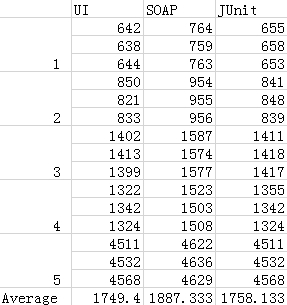
\includegraphics[width=6cm,height=6cm,keepaspectratio]{img/timeTable.jpg}
\caption{Time taken by different approaches}
\label{overflow}
\end{figure}


Figure 6 illustrates the average time taken every test case:\\

\begin{figure}[ht!]
\centering
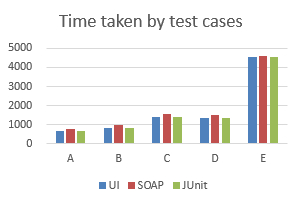
\includegraphics[width=9cm,height=9cm,keepaspectratio]{img/timeGraph.jpg}
\caption{Time taken by test cases}
\label{overflow}
\end{figure}

The graph shows that all three approaches finish all test cases in the same time frame with SOAP taking the longest and JUnit taking the least. This result is reasonable since the amount of time that runtime execution takes is dominant in the values displayed on the graph. At the mean time, the SOAP protocol wraps input data in an envelope when sending and checks the output with assertions and validations. This can explain the fact that it is taking longer than the others. Please note that this subsection does not measure the amount of time for quality analysts to enter the data when using the three approaches. This justified in the next subsection. \\


\subsection{Automation}
Automation is the most popular topic among quality analysts who seek to improve their testing. Testing automation is a technique that boosts efficiency and reduces human labour. A large number of test cases are controlled by the system and run against the web application automatically when a test command is generated by the tester or when the application is built.\\

The first approach is the least automation friendly approach, considering that data is entered from the UI. Although it is possible using a language such as Python, this is not encouraged or practically viable. The reason is that VIP room is an enterprise web application with thousands of customers. The security layer that wraps the application redundantly checks if the data is entered by some artificial intelligence to prevent brute force security penetration. Therefore automated testing is not feasible for this approach.\\

The possibility for automated SOAP testing solely depends on the software used. Some light weight SOAP software (or web client) does not have automation features. However in SoapUI, test cases are managed to be automation ready. It means that test cases are grouped and named so a particular group of cases can be extracted and run against the application instantly. The group and number of cases are controlled by the tester.

\begin{figure}[ht!]
\centering
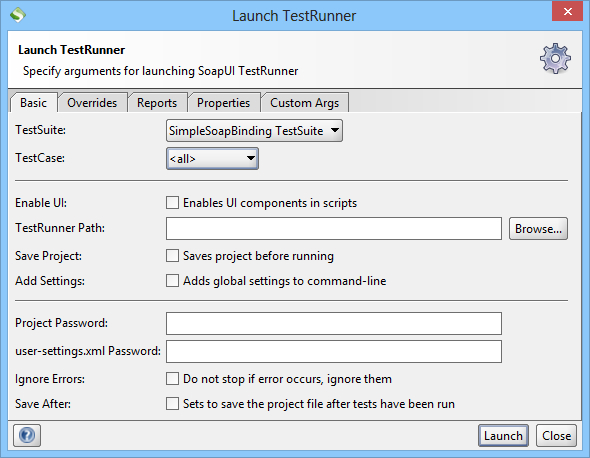
\includegraphics[width=12cm,height=12cm,keepaspectratio]{img/soapAuto.jpg}
\caption{SoapUI automation feature}
\label{overflow}
\end{figure}

The window above is SoapUI's interface for automation testing. Although it does save the tester a lot of time and reduce the chance for mistakes, it is still not completely automated in the sense that it still needs to be configured and launched manually every time. True automation requires no human efforts after the initial test case configuration.\\

One of the advantages JUnit has is that it is integrated in the Maven build process. “Apache Maven is a software project management and comprehension tool. Based on the concept of a project object model (POM), Maven can manage a project's build, reporting and documentation from a central piece of information.”\cite{maven} The VIP room web application uses Maven as its build manager. Every time a complete build (tests can be skipped to save build time) is done, the JUnit test cases are automatically run against the application. should any test fail, detail error message will be displayed in the console and the build will be marked as unsuccessful. As previously explained, JUnit “tests the smallest piece of testable software in the application.”\cite{unit} This means that JUnit test cases are likely to be static as shown by the code block on page 6. This defeats the definition of functional testing, which should cover all permutation of scenario. In order to cope with this, a test controller is needed to wrap the JUnit test cases to form a dynamic test. Here is a modified version of Java Class Simple:

\begin{lstlisting}
// Simple.java

public class Simple {
	public int add(int a, int b){
		return a + b;
	}
	
	public int subtract(int a, int b){
		return a - b;
	}
	
	public int multiply(int a, int b){
		return a * b;
	}
}
\end{lstlisting}

\subsection{Reproduction}
\subsection{Customization}
\subsection{Management}


\section{Conclusions}
CONCLUSIONS


\section{Recommendations}
RECOMMENDATIONS


\newpage


\addcontentsline{toc}{section}{\refname}
\bibliography{wkrpt}
\begin{thebibliography}{1}

  \bibitem{telusComp} Telus Health Inc., "Telus Health: Home," Telus Health Inc., {\em http://www.telushealth.com/} (current April 11 2014).

  \bibitem{soap} W3C Note, "Simple Object Access Protocol (SOAP) 1.1," W3C Note, {\em http://www.w3.org/TR/2000/NOTE-SOAP-20000508/} (current April 11 2014).

\bibitem{unit} Microsoft Corp., "Unit Testing," MSDN - Microsoft, {\em http://msdn.microsoft.com/en-us/library/aa292197(v=vs.71).aspx} (current April 11 2014).

\bibitem{maven} Apache Foundation., "Maven," Apache Foundation, {\em http://maven.apache.org/} (current April 11 2014).

\end{thebibliography}
\newpage


\tocsection{Acknowledgements}
ACKNOWLEDGEMENTS
\newpage


% \appendix{APPENDIX INDEX}{APPENDIX NAME}
% APPENDICES
% \newpage


\end{document}

